\documentclass[uplatex]{jsarticle}
\usepackage{amsmath}
\usepackage{amssymb}
\usepackage{amsthm}
\usepackage{framed}
\usepackage[dvipdfmx]{graphicx,xcolor}
\usepackage{tikz}
\usetikzlibrary{calc}

\newcommand{\N}{\mathbb{N}}
\newcommand{\Z}{\mathbb{Z}}
\newcommand{\Q}{\mathbb{Q}}
\newcommand{\R}{\mathbb{R}}

\begin{document}
	
	\thispagestyle{empty}

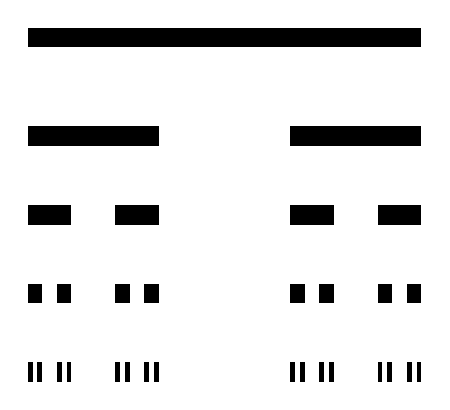
\begin{tikzpicture}[scale = 5]
\fill (0,0) rectangle (1,0.05);

\fill (0/3,-0.2) rectangle (1/3,-0.2-0.05);
\fill (2/3,-0.2) rectangle (3/3,-0.2-0.05);

\fill (0/9,-0.2*2) rectangle (1/9,-0.2*2-0.05);
\fill (2/9,-0.2*2) rectangle (3/9,-0.2*2-0.05);
\fill (6/9,-0.2*2) rectangle (7/9,-0.2*2-0.05);
\fill (8/9,-0.2*2) rectangle (9/9,-0.2*2-0.05);

\fill (0/27,-0.2*3) rectangle (1/27,-0.2*3-0.05);
\fill (2/27,-0.2*3) rectangle (3/27,-0.2*3-0.05);
\fill (6/27,-0.2*3) rectangle (7/27,-0.2*3-0.05);
\fill (8/27,-0.2*3) rectangle (9/27,-0.2*3-0.05);
\fill (18/27,-0.2*3) rectangle (19/27,-0.2*3-0.05);
\fill (20/27,-0.2*3) rectangle (21/27,-0.2*3-0.05);
\fill (24/27,-0.2*3) rectangle (25/27,-0.2*3-0.05);
\fill (26/27,-0.2*3) rectangle (27/27,-0.2*3-0.05);

\fill (0/81,-0.2*4) rectangle (1/81,-0.2*4-0.05);
\fill (2/81,-0.2*4) rectangle (3/81,-0.2*4-0.05);
\fill (6/81,-0.2*4) rectangle (7/81,-0.2*4-0.05);
\fill (8/81,-0.2*4) rectangle (9/81,-0.2*4-0.05);
\fill (18/81,-0.2*4) rectangle (19/81,-0.2*4-0.05);
\fill (20/81,-0.2*4) rectangle (21/81,-0.2*4-0.05);
\fill (24/81,-0.2*4) rectangle (25/81,-0.2*4-0.05);
\fill (26/81,-0.2*4) rectangle (27/81,-0.2*4-0.05);

\fill (54/81,-0.2*4) rectangle (55/81,-0.2*4-0.05);
\fill (56/81,-0.2*4) rectangle (57/81,-0.2*4-0.05);
\fill (60/81,-0.2*4) rectangle (61/81,-0.2*4-0.05);
\fill (62/81,-0.2*4) rectangle (63/81,-0.2*4-0.05);
\fill (72/81,-0.2*4) rectangle (73/81,-0.2*4-0.05);
\fill (74/81,-0.2*4) rectangle (75/81,-0.2*4-0.05);
\fill (78/81,-0.2*4) rectangle (79/81,-0.2*4-0.05);
\fill (80/81,-0.2*4) rectangle (81/81,-0.2*4-0.05);
\end{tikzpicture}

\end{document}
